% Chapter Template
\tocdata{toc}{Terence Tan}

\chapter{Training Data \& Data Processor} % Main chapter title

\label{Chapter3} % Change X to a consecutive number; for referencing this chapter elsewhere, use \ref{ChapterX}

As illustrated in \autoref{fig:MVPOverview}, the data from the voice processor will be passed to a data processor to convert it into the appropriate input data format for the machine learning model. But before that, the model has to be trained first in order to be of any use. Hence, we shall look at the dataset used to train and test the model before discussing the data processor in Section \ref{data processor}.

The processing of the raw dataset into the training/testing dataset had been carried out; as mentioned in \autoref{Project management}, the code and resulting datasets can be found on our git repository \footnote{https://github.com/edsgunn/TerrenceInABox}. The data processor itself has not been coded but would be easy to create by re-using the code used to process the raw dataset.
%----------------------------------------------------------------------------------------
%	SECTION 1
%----------------------------------------------------------------------------------------

\section{Dataset}
\label{Intro to Dataset}
Papers that worked on similar chord generation problems \cite{MySong} \cite{BLSTM} \cite{MLForChords} obtained their dataset by collecting lead sheets from public and private sources and preprocessing them. Unfortunately, most of them did not publicly share their processed dataset. We could collect and preprocess our own lead sheets, of which there are quite a few possible sources such as MuseScore and the Million Song Dataset \cite{Bertin-Mahieux2011}. However, \cite{BLSTM} do provide their preprocessed dataset in which the features of the lead sheets have already been extracted. Given that extracting the musical features ourselves would be time-consuming, and that we are building a Minimum Viable Product that would not require an extensive dataset, we decided to use that dataset.

There are 2252 songs in this dataset, 1802 of which had been categorised as the training set while the remaining 450 had been categorised as the test set. Each song is in major key and only have a single chord per bar. For each song, all the relevant features had been extracted and placed into a single \emph{CSV} file. These files can then be read and converted to DataFrame format using Python \emph{Pandas} as shown in Figure \ref{fig:CSV_DF}.

As can be seen in Figure \ref{fig:CSV_DF}, the rows each contain information about a single note. Each bar is taken to be a single measure. The columns each represent a different piece of information about that particular note. \emph{time} refers to the time signature, \emph{measure} refers to the measure to which that particular note belongs to, \emph{key\_fifths} indicates the number of sharps/flats (e.g. -1 for one flat and 1 for one sharp), \emph{chord\_root} is the root of the chord with \emph{chord\_type} indicating the type of chord, \emph{note\_root} identifies the particular single note of that row, \emph{note\_octave} is the octave of that note, and \emph{note\_duration} indicated the duration of the note (4.0 for a quarter note).

\begin{figure}
\centering
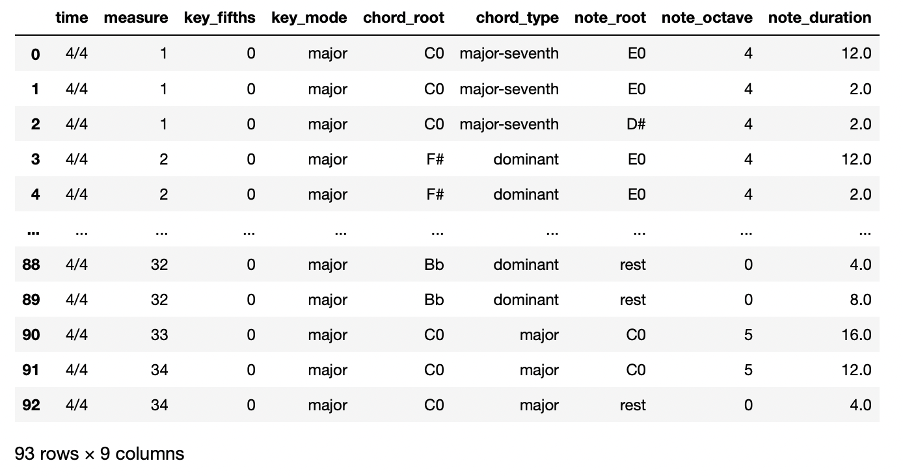
\includegraphics{Figures/CSV dataframe}
\decoRule
\caption{A song in DataFrame format after being read from CSV file}
\label{fig:CSV_DF}
\end{figure}

%-----------------------------------
%	SECTION 2
%-----------------------------------
\section{Preprocessing of dataset}
\label{preprocessing}

The dataset can be preprocessed to remove unnecessary information in order to make the dataset cleaner and ready for conversion into input formats that are compatible with our machine learning models. Steps 1-5 listed below are based on the preprocessing done in the other papers that worked on similar chord generation problems \cite{MySong} \cite{BLSTM} \cite{MLForChords}. We paid particular attention to the preprocessing steps of the paper \cite{BLSTM} from which we obtained our dataset.

\begin{enumerate}
  \item All songs are transposed to C major key. The key of a song determines the notes and the set of chords present in the song. Transposing all songs to a common key will normalise the different features of melodies and chords in different songs. The number of chord types present in the dataset will be reduced, which will decrease the number of chord types during the training process. Each song can be shifted to a different key without loss of the song's subjective character by shifting all the pitches equally \cite{MySong} \cite{MLForChords} \cite{BLSTM}.
  \item The time signatures are all normalised. Since different songs have different time signatures, each \emph{note\_duration} is multiplied by the reciprocal of the time signature \emph{time} to give a normalised note duration \cite{BLSTM}.
  \item Chord types are restricted to major and minor chords since having all chord types exist as independent classes will result in too few datapoints for each chord type \cite{BLSTM}. All other chord types are converted to their most similar major or minor chords by simplifying them to their core triads. This would result in loss of some emotive character, but would not sigficantly degrade the appropriateness of a chord for a particular melody segment \cite{MySong}. Note that more chord types can be easily added to our model in the future by adding more columns to the data input matrix in Section \ref{LSTM format for training} and by including more class types in the chord sequence in Section \ref{Transformer format for training}.
  \item Some measures in the dataset contain rest notes. These measures can be removed from the dataset \cite{MLForChords}.
  \item Octave information is not required and is removed from the dataset \cite{BLSTM}.
  \item There are also some irregular notes present in the dataset such as 'B-2' and 'A2' as shown in Figure \ref{fig:notefreq} using the \emph{value\_counts()} function. Further analysis shows that the numbers after the letters do not seem to represent octave or any other information; as can be seen in Figure \ref{fig:irregnote}, the indexed measures all have a \emph{note\_root} of 'B\-2' but do not all share a commonality in any of the other columns (excluding \emph{key\_mode} which would be 'major' for all measures since the dataset only contains songs in the major key). The paper from which this dataset was obtained also made no mention of these irregular notes. Given that they represent a very small portion of the dataset (41 measures as calculated from Figure \ref{fig:notefreq}), measures containing these irregular notes are removed.
\end{enumerate}

\begin{figure}
    \centering
    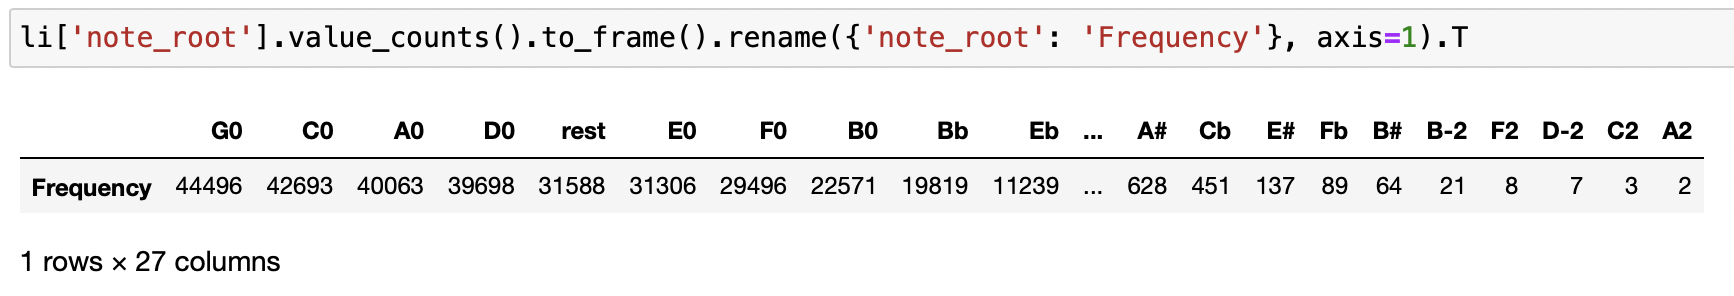
\includegraphics[scale=0.5]{Figures/note frequency}
    \decoRule
    \caption{Number of each \emph{note\_root} (frequency) that exists within the entire dataset.}
    \label{fig:notefreq}
    \end{figure}
    
    \begin{figure}
        \centering
        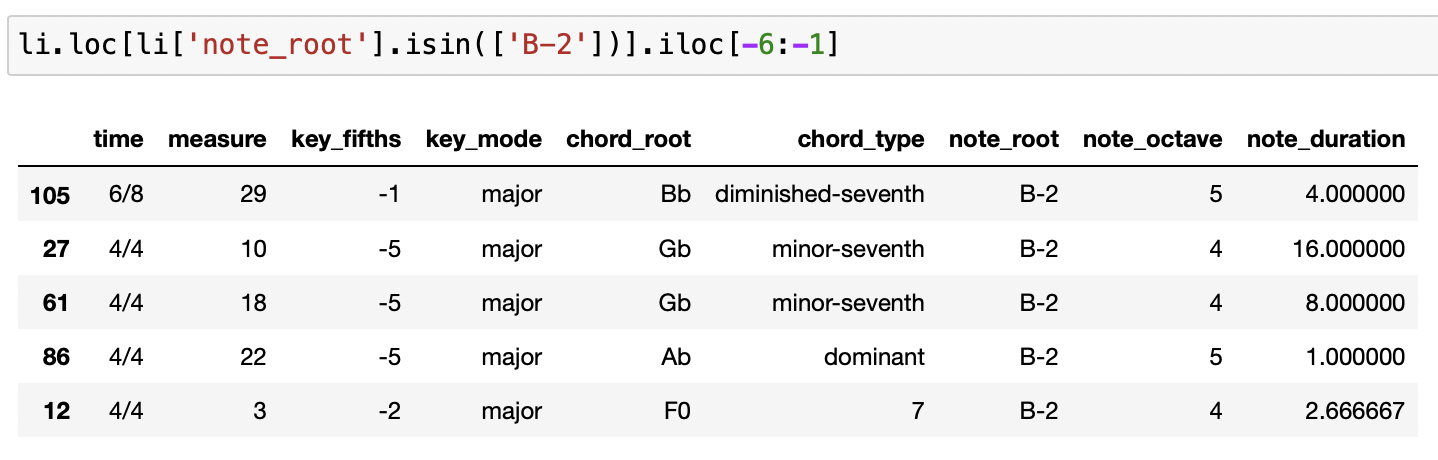
\includegraphics[scale=0.5]{Figures/irregular notes}
        \decoRule
        \caption{Indexed measures containing \emph{note\_root} of 'B\_2'.}
        \label{fig:irregnote}
        \end{figure}
        
%-----------------------------------
%	SUBSECTION 1
%-----------------------------------
A pictorial representation of the steps above can be found in Figure \ref{fig:Alg1}. It might be useful to refer to that figure as we go into details about the preprocessing below.

Using \emph{Pandas} to remove the unwanted measures mentioned above and to normalise the note durations is a straightforward task. However, shifting all the songs to C major key is trickier. We would need to know the original key of the song, and then transposed the \emph{note\_root} and \emph{chord\_root} appropriately to C major key. The original keys of the songs are stated implicitly by their \emph{key\_fifths}; since we know all the songs are in major key and that each major key has a unique number of sharps/flats, the numberical value of \emph{key\_fifths} can be mapped to a specific major key as shown in Table \ref{tab:kf_map}. Note that there exist more values of \emph{key\_fifths} than shown, but preliminary analysis of the dataset shows that only integer values of \emph{key\_fifths} from -6 to 7 are present within it. We also create a mapping of the 12 notes to a numerical representation as shown in Table \ref{tab:note_map} to make the processing easier later.

Using Table \ref{tab:kf_map} \& \ref{tab:note_map}, we can list all the major keys present in the dataset and convert the pitches that exist within each major key into their numerical representations (which goes from 1 to 12 and then loops back to 1) as shown in Table \ref{tab:bigtable}. As expected, the differences between the pitches of the same key are consistent across all the major keys (e.g. the difference between Pitch 1 and Pitch 3 is always 4 for every major key), which shows that we can indeed tranpose a song to a different key by just shifting all the pitches equally. For each DataFrame row, we just have to convert \emph{key\_fifths} to the corresponding major key using \autoref{tab:kf_map} to obtain the numerical representaion of Pitch 1 of that major key. We also convert \emph{note\_root} and \emph{chord\_root} to numbers using Table \ref{tab:note_map}. Next, the numerical representation of Pitch 1 $p_1$ is subtracted from those of \emph{note\_root} $n_r$ and \emph{chord\_root} $c_r$, and the differences are added to Pitch 1 of the C major key $p_{1,c}$ (which is equal to 1) to obtain the shifted pitches in notes $n_{r,shifted}$ and chords $c_{r,shifted}$ respectively: 

\begin{align} 
    \label{shift note 1}
    n_{r,shifted} = (n_r-p_1)+p_{1,c} = (n_r-p_1)+1\\
    \label{shift chord 2}
    c_{r,shifted} =(c_r-p_1)+p_{1,c} = (c_r-p_1)+1
\end{align}
where $n_r$ and $c_r$ are the original note and chord respectively, $p_1$ is Pitch 1 of the original key of the song, and $p_{1,c}$ is Pitch 1 of C major key.

Note that the differences may be negative, which would lead to a shifted note/chord that is outside the 1-12 range. This is easily rectified by using \emph{if} statements to check if the shifted note/chord is non-positive and to add 12 (since the numerical representations loop back to 1 after 12) to it if so. This gives us:

\begin{align}
    \label{shift note 2}
    n_{r,shifted}= 
\begin{cases}
    (n_r-p_1)+1,& \text{if } n_r > p_1-1\\
    (n_r-p_1)+13,              & \text{otherwise}
\end{cases}\\
c_{r,shifted}= 
\begin{cases}
    (c_r-p_1)+1,& \text{if } c_r > p_1-1\\
    (c_r-p_1)+13,              & \text{otherwise}
\end{cases}
\end{align}

The next step is to convert all the chord types to either major or minor chords using the mapping shown in Table \ref{tab:chords}. This mapping has been checked by the supervisors of this project and deemed to be reasonable. Do also note that Table \ref{tab:chords} does not contain an exhaustive list of all chords in existence, but only those that were found to be present within the dataset.

\subsection{Code}
As mentioned above, we first use \emph{Pandas} to clean up the data. A nested loop can then be used to loop through each DataFrame row for each song. The steps outlined above in Chapter \ref{preprocessing} can then be applied to each row. At the end of the nested loop, the dataset is now fully preprocessed.

%\begin{figure}
 %   \centering
  %  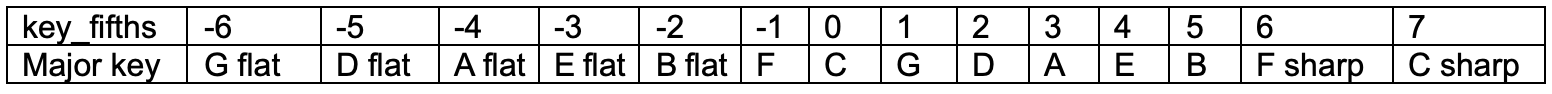
\includegraphics{Figures/key_fifths_mapping}
   % \decoRule
   % \caption{Mapping of \emph{key\_fifths} to major key}
   % \label{fig:kf_map}
    %\end{figure}

    \begin{table}
        \caption{Mapping of \emph{key\_fifths} to major key}
        \label{tab:kf_map}
        \centering
        \begin{tabular}{|c||c|c|c|c|c|c|c|c|c|c|c|c|c|c|}
        \hline
        \emph{key\_fifths} & -6 & -5 & -4 & -3 & -2 & -1 & 0 & 1 & 2 & 3 & 4 & 5 & 6 & 7 \\
        \hline
        Major key & Gb & Db & Ab & Eb & Bb & F & C & G & D & A & E & B & F\# & C\# \\
        \hline
        \end{tabular}
        \end{table}

\begin{table}
    \caption{Mapping of music notes to numerical representations}
    \label{tab:note_map}
    \centering
    \begin{tabular}{|c|c|c|c|c|c|}
    \hline
    C/B\# & C\#/Db & D & D\#/Eb & E/Fb & F/E\# \\
    \hline
    1 & 2 & 3 & 4 & 5 & 6 \\
    \hline
    \end{tabular}
    \begin{tabular}{|c|c|c|c|c|c|}
        \hline
    F\#/Gb & G & G\#/Ab & A & A\#/Bb & B/Cb\\
    \hline
    7 & 8 & 9 & 10 & 11 & 12\\
    \hline
    \end{tabular}
    \end{table}

    \begin{table}
        \caption{The component notes/pitches of each major key}
        \label{tab:bigtable}
        \centering
        \begin{tabular}{|c||c|c|c|c|c|c|c|}
        \hline
        Major key & Pitch 1 & Pitch 2 & Pitch 3 & Pitch 4 & Pitch 5 & Pitch 6 & Pitch 7 \\
        \hline
        \hline
        C\# & 2 & 4 & 6 & 7 & 9 & 11 & 1 \\
        \hline
        F\# & 7 & 9 & 11 & 12 & 2 & 4 & 6\\
        \hline
        B & 12 & 2 & 4 & 5 & 7 & 9 & 11\\
        \hline
        E & 5 & 7 & 9 & 10 & 12 & 2 & 4\\
        \hline
        A & 10 & 12 & 2 & 3 & 5 & 7 & 9\\
        \hline
        D & 3 & 5 & 7 & 8 & 10 & 12 & 2\\
        \hline
        G & 8 & 10 & 12 & 1 & 3 & 5 & 7\\
        \hline
        C & 1 & 3 & 5 & 6 & 8 & 10 & 12\\
        \hline
        F & 6 & 8 & 10 & 11 & 1 & 3 & 5\\
        \hline
        Bb & 11 & 1 & 3 & 4 & 6 & 8 & 10\\
        \hline
        Eb & 4 & 6 & 8 & 9 & 11 & 1 & 3\\
        \hline
        Ab & 9 & 11 & 1 & 2 & 4 & 6 & 8\\
        \hline
        Db & 2 & 4 & 6 & 7 & 9 & 11 & 1\\
        \hline
        Gb & 7 & 9 & 11 & 12 & 2 & 4 & 6\\
        \hline
        \end{tabular}
        \end{table}

        \begin{table}
            \caption{Mapping of chords present within the dataset to major/minor chord.}
            \label{tab:chords}
            \centering
            \begin{tabular}{l l}
            \toprule
            Major & Minor \\
            \midrule
            Dominant-ninth & Minor-seventh\\
            Major-sixth & Minor-sixth\\
            Major-seventh & Diminished\\
            Dominant & Half-diminished\\
            Suspended-fourth & Minor-ninth\\
            Augmented-seventh & Diminished-seventh\\
            Major-ninth & Minor-eleventh\\
            Dominant-seventh & Minor-major\\
            Augmented & Major-minor\\
            Dominant-thirteenth & Minor-thirteenth\\
            Power & Minor seven flat five\\
            Suspended-second &  \\
            Dominant-eleventh &  \\
            Pedal &  \\
            Major 6/9 &  \\
            Augmented-ninth &  \\
            Sixth &  \\

            \bottomrule\\
            \end{tabular}
            \end{table}
            

        \begin{figure}
            \centering
            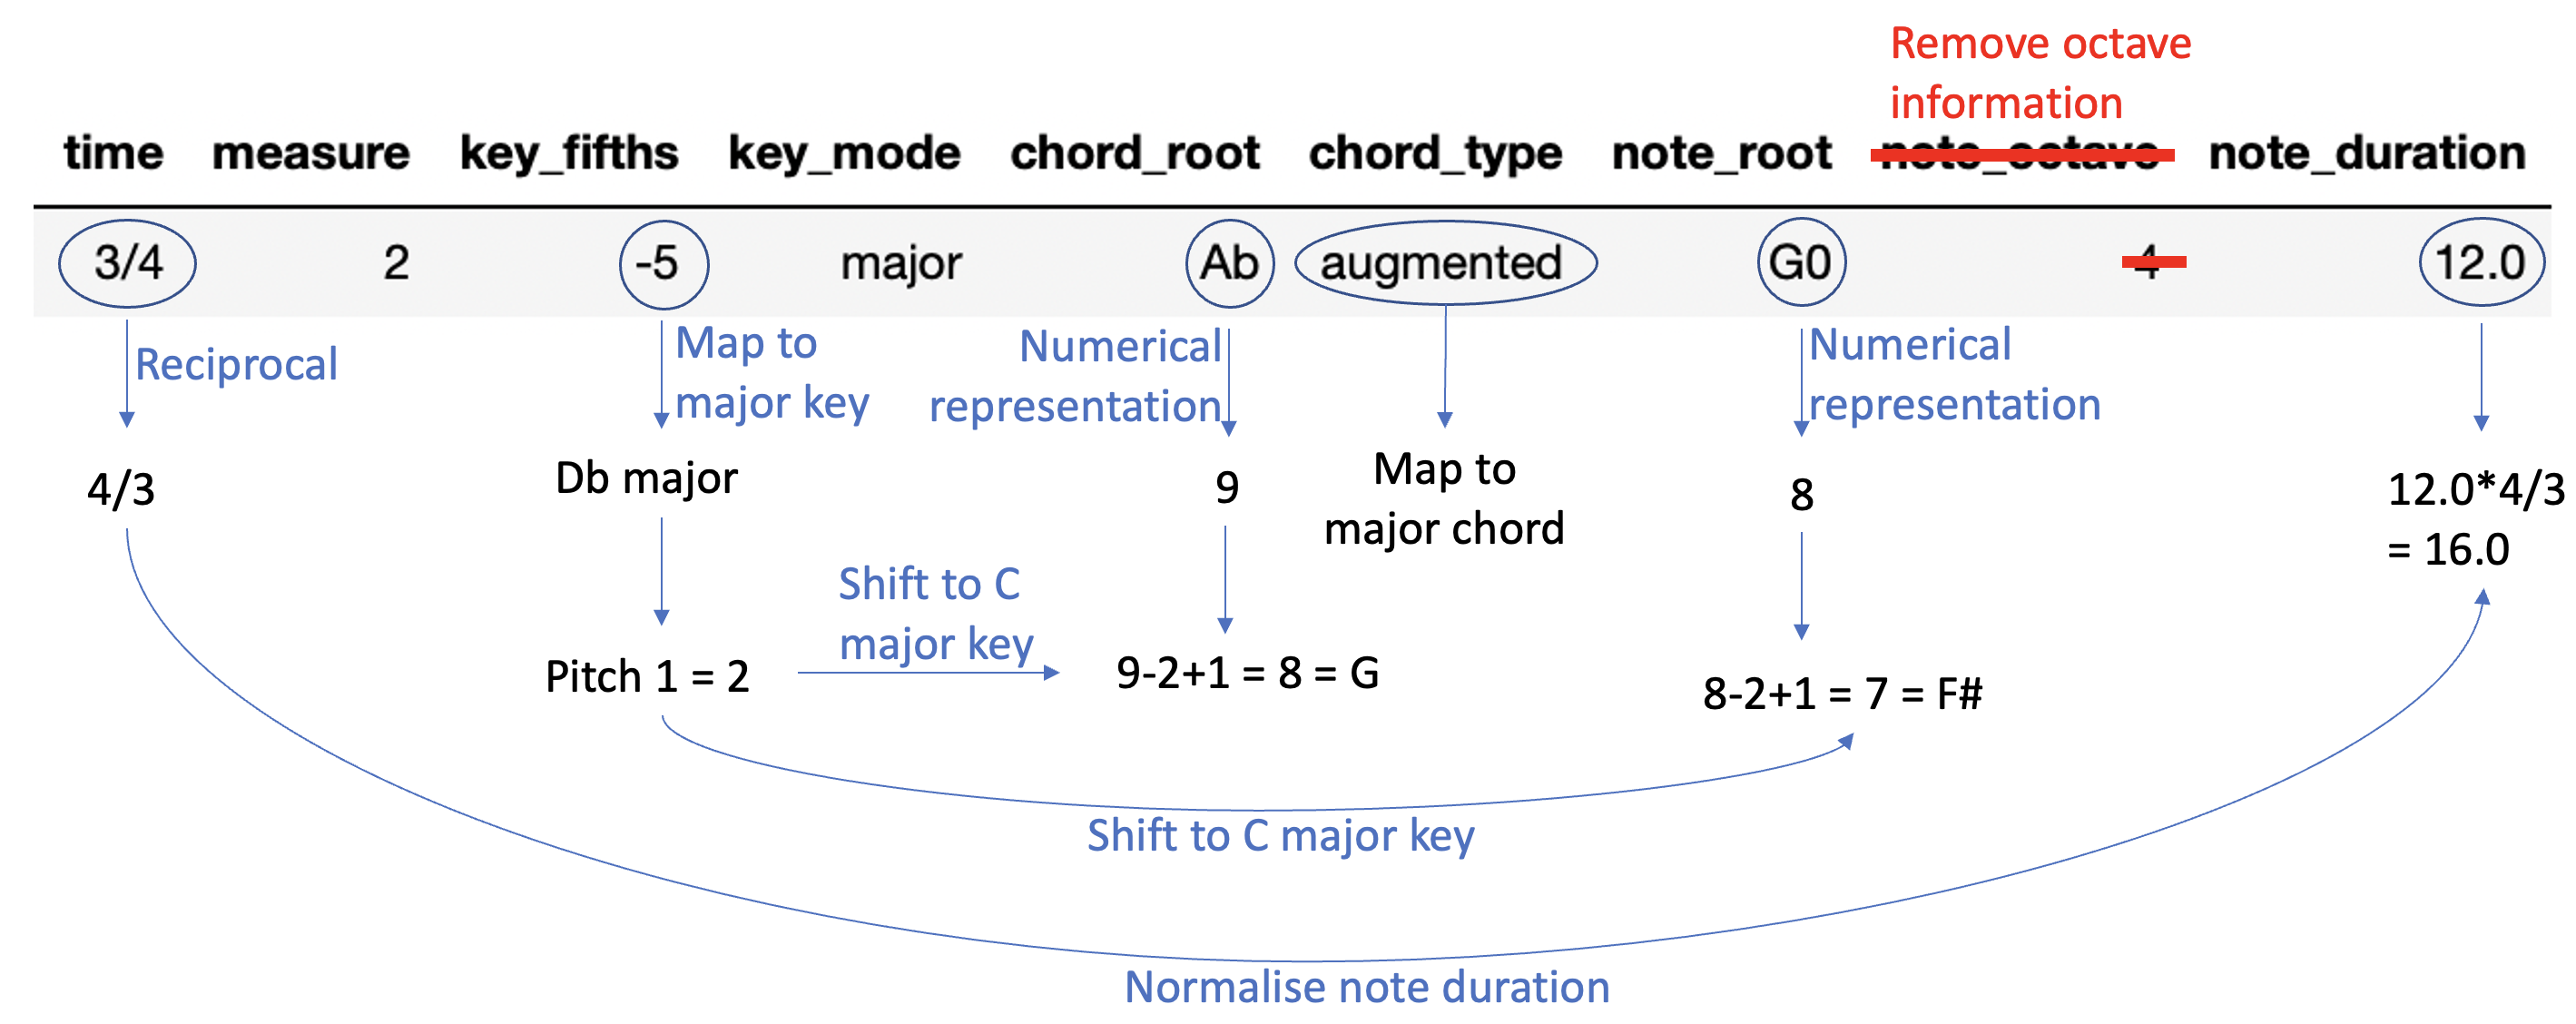
\includegraphics[scale=0.3]{Figures/Algorithm pictorial2}
            \decoRule
            \caption{Pictorial representation of the preprocessing of the dataset.
            }
            \label{fig:Alg1}
            \end{figure}
            
%-----------------------------------
%	SUBSECTION 2
%-----------------------------------

%\subsection{Subsection 2}
%Morbi rutrum odio eget arcu adipiscing sodales. Aenean et purus a est pulvinar pellentesque. Cras in elit neque, quis varius elit. Phasellus fringilla, nibh eu tempus venenatis, dolor elit posuere quam, quis adipiscing urna leo nec orci. Sed nec nulla auctor odio aliquet consequat. Ut nec nulla in ante ullamcorper aliquam at sed dolor. Phasellus fermentum magna in augue gravida cursus. Cras sed pretium lorem. Pellentesque eget ornare odio. Proin accumsan, massa viverra cursus pharetra, ipsum nisi lobortis velit, a malesuada dolor lorem eu neque.

%----------------------------------------------------------------------------------------
%	SECTION 3
%----------------------------------------------------------------------------------------

\section{Model input format}
\label{Model input format}
Now that the dataset has been preprocessed, it can now be converted into a format that is appropriate for input to our machine learning model which, as will be stated in \autoref{Our Model}, is a conditional Generative Adversarial Network with Long Short Term Memory \(LSTM\) layers; we shall refer to this model simply as LSTM for the rest of this chapter. In addition, we shall also discuss the data format of the Transformer, which is another strong candidate for the machine learning model that can be tested against the LSTM in future extensions of this project. Hence, we will convert the data into formats that are appropriate for two models: the LSTM and the Transformer.

\subsection{LSTM format}
\label{LSTM format for training}
The LSTM data input format is a matrix with 37 columns, with each row containing information about a single measure. The first 12 columns represent the 12 note (C, C\#, etc.), the next 24 columns represent the 12 major chords and the 12 minor chords, and the last column corresponds to the absence of a chord. If a particular note exists within a particular measure, the element that corresponds to that particular measure (row) and particular note (column) will be the normalised duration of that note. Similarly, the element that corresponds to the chord of a particular measure will be a '1'. Notes and chords that are not present within that measure will be marked with a '0'. If no chords are present within a measure, the last column will be marked as a '1'. A pictorial representation of the transformation is shown in Figure \ref{fig:LSTM training}.

\subsubsection{Code}
We again use a nested loop to loop through each DataFrame row for each song. Two 1 by 37 arrays \emph{LSTM\_data} and \emph{new\_row} are initialised. As we loop through each row, we keep track of the measure. As long as the measure does not change, \emph{new\_row} is progressively updated with the normalised note durations of the present notes in this manner: 
\begin{equation}  
\emph{new\_row}[0,\emph{note}-1] = \emph{new\_row}[0,\emph{note}-1] + \emph{normalised\_note\_duration},
\end{equation}
where \emph{note} is the numerical representation of the note present in each DataFrame row and \emph{normalised\_note\_duration} is the normalised note duration of that note. 

This works because the mapping between the notes and their numerical representation starts at 1 and ends at 12 (as can be seen in Table \ref{tab:note_map}) and indexing starts at zero in Python. Hence, the (\emph{note}-1)\textsuperscript{th} column of the LSTM format (and thereby \emph{new\_row}) will correspond to \emph{note}.

Once the measure changes, the now complete \emph{new\_row} for the previous measure is concatenated with \emph{LSTM\_row} along the row axis, i.e. \emph{new\_row} is added to the bottom of \emph{LSTM\_row}. The elements of \emph{new\_row} are reset to zero before \emph{new\_row} is updated with the note and chord information of the current measure. The note information can be updated as explained earlier. For the chord information, we can use \emph{if} statements to set $\emph{new\_row}[0, \emph{chord}+11] = 1$ if \emph{chordtype} = 'major', or to set $\emph{new\_row}[0, \emph{chord}+23] = 1$ if \emph{chordtype} = 'minor', or to set $\emph{new\_row}[0, -1] = 1$ otherwise (no chord present), where \emph{chord} is the numerical representation of \emph{chord\_root} (mapped using Table \ref{tab:note_map}). Since we know that there is only one chord type per measure, we only have to update the chord information for \emph{new\_row} once, at the start of a new measure. The start of the first measure can be taken to be a special case of a measure change (in this case, transition from a measure initialised as 'unknown' to the first measure of the DataFrame).

Note that we could have combined this section with the preprocessing steps in Chapter \ref{preprocessing} such that we only have to loop through each DataFrame row for each song once instead of doing it twice as we actually did. This would have reduced the time needed to run the entire code by eliminating redundant loops. However, the time saved for a dataset of this size is insignificant. Additionally, keeping the two code blocks separate made it easier to test and debug, which is why we decided not to integrate them together. Nonetheless, integration of the code is definitely something to take into consideration for any future extensions of this project.
%$\emph{new\_row}[0,\emph{note}-1] = \emph{new\_row}[0,\emph{note}-1] + \emph{normalised\_note\_duration}$
\begin{figure}
    \centering
    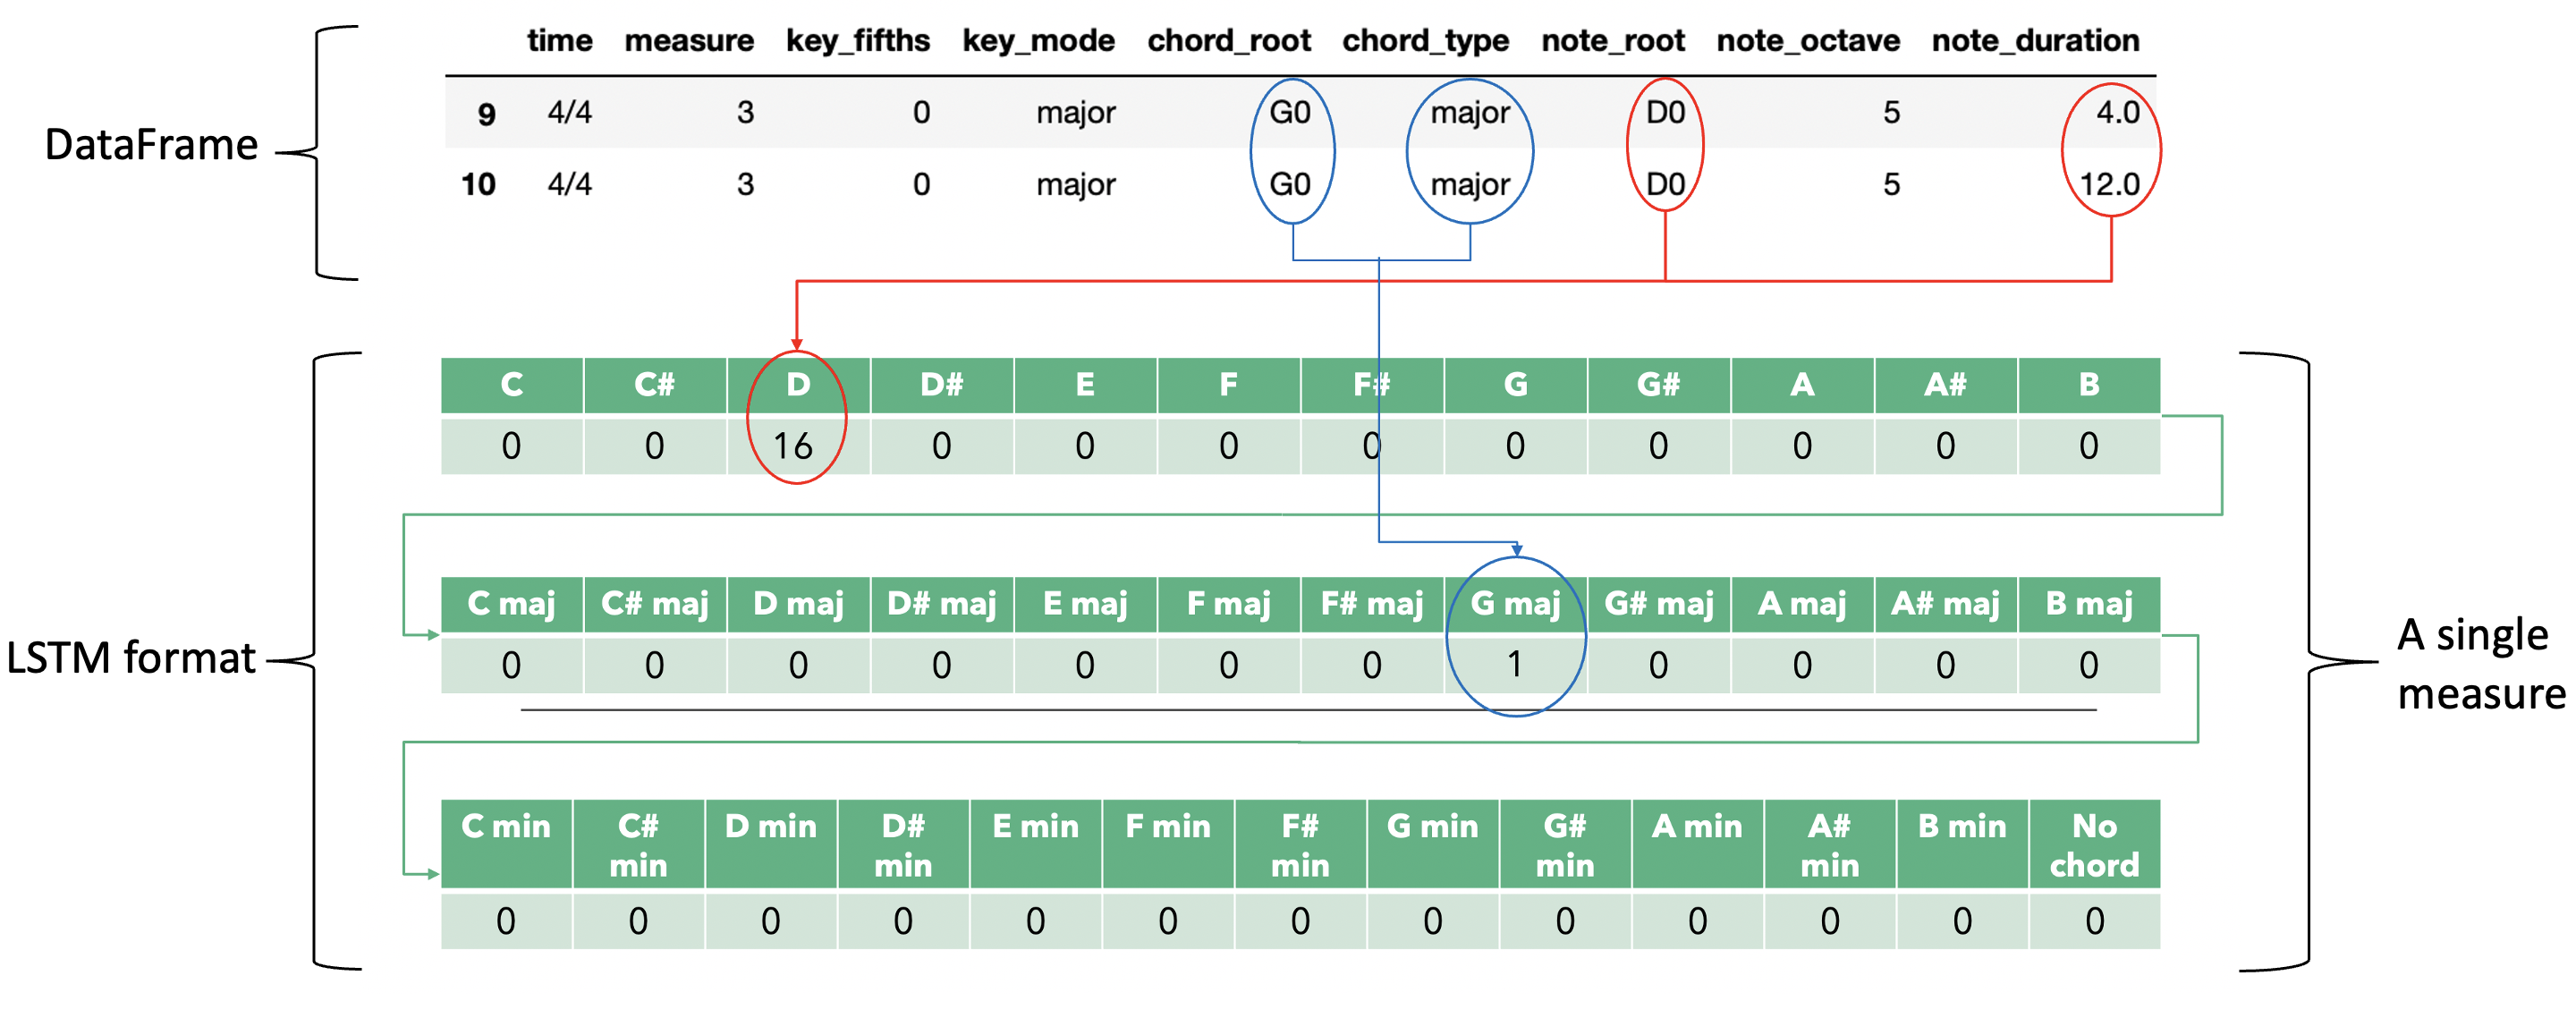
\includegraphics[scale=0.3]{Figures/LSTM pictorial 4}
    \decoRule
    \caption{Transforming DataFrame to LSTM data input format.}
    \label{fig:LSTM training}
    \end{figure}
    
\subsubsection{Sanity Check of code}
\label{lstm check}
We know that each row of the LSTM data input format corresponds to a single measure. We also know that the preprocessing done in Chapter \ref{preprocessing} would have removed unnecessary measures from some songs. Hence, the LSTM data cannot possibly have more measures than the original dataset for each song. By comparing the number of rows of the LSTM data and the highest value of \emph{measure} in the original Dataframe for each song, we can perform a simple check of the correctness of our code. From Figure \ref{fig:LSTM check}, we can see that no songs in LSTM data input format has more measures than in their original DataFrame format.

In addition, we picked out a few songs at random and manually checked the format conversion.

\begin{figure}
    \centering
    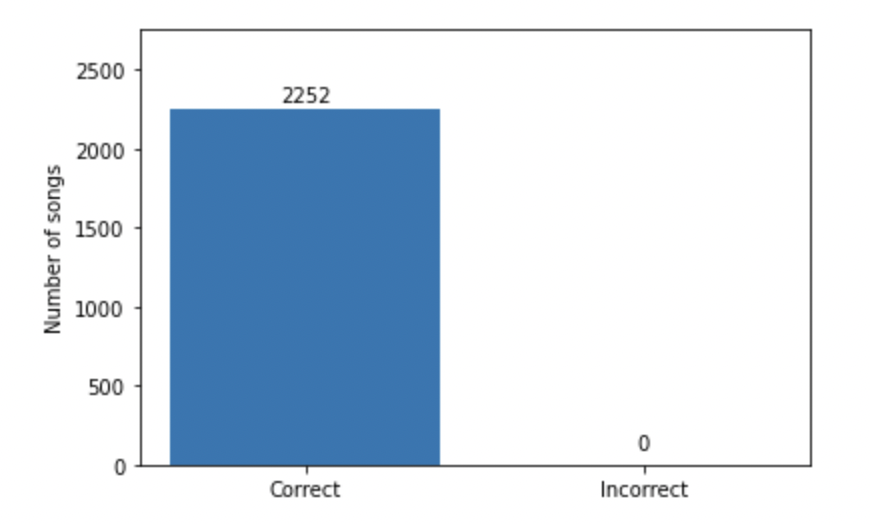
\includegraphics{Figures/LSTM check}
    \decoRule
    \caption{Number of songs in LSTM format with 'correct' and 'incorrect' number of measures.}
    \label{fig:LSTM check}
    \end{figure}

\subsection{Transformer format}
\label{Transformer format for training}
The transformer requires two data inputs: a single sequence of notes for each song, and a separate sequence of chords for each song. Both sequences are constructed by going down the Dataframe rows, and adding the notes/chords of each row to the respective sequences based on the \emph{note\_duration} value, e.g. a sequence of 4 'C\#'s for a 'C\#' with a \emph{note\_duration} of 4.0, and a sequence of 16 'Bmaj's for a 'B major' of \emph{note\_duration} of 16.0. Another example is presented in Figure \ref{fig:Transformer training}. This means that only integer values of \emph{note\_duration} are accepted and measures with non-integer values have to be removed beforehand.

It is obvious that the sequences will be very long given that just the three rows in Figure \ref{fig:Transformer training} resulted in 16 elements for each sequence. As shown in Chapter 4, the time complexity of the Transformer is $O({n}^2)$. Hence, it is crucial to reduce the sequence length to shorten the training time. This can be achieved by dividing all \emph{note\_duration} by their largest common factor for all measures within a single song. This may not reduce the length of the sequences for all songs (songs with \emph{note\_duration of 1.0} will have a trivial largest common factor of 1.0), but it will still reduce the sequence length for some songs, as shown in Figure \ref{fig:Transformer LCF}, which will decrease the training time significantly.


\begin{figure}
    \centering
    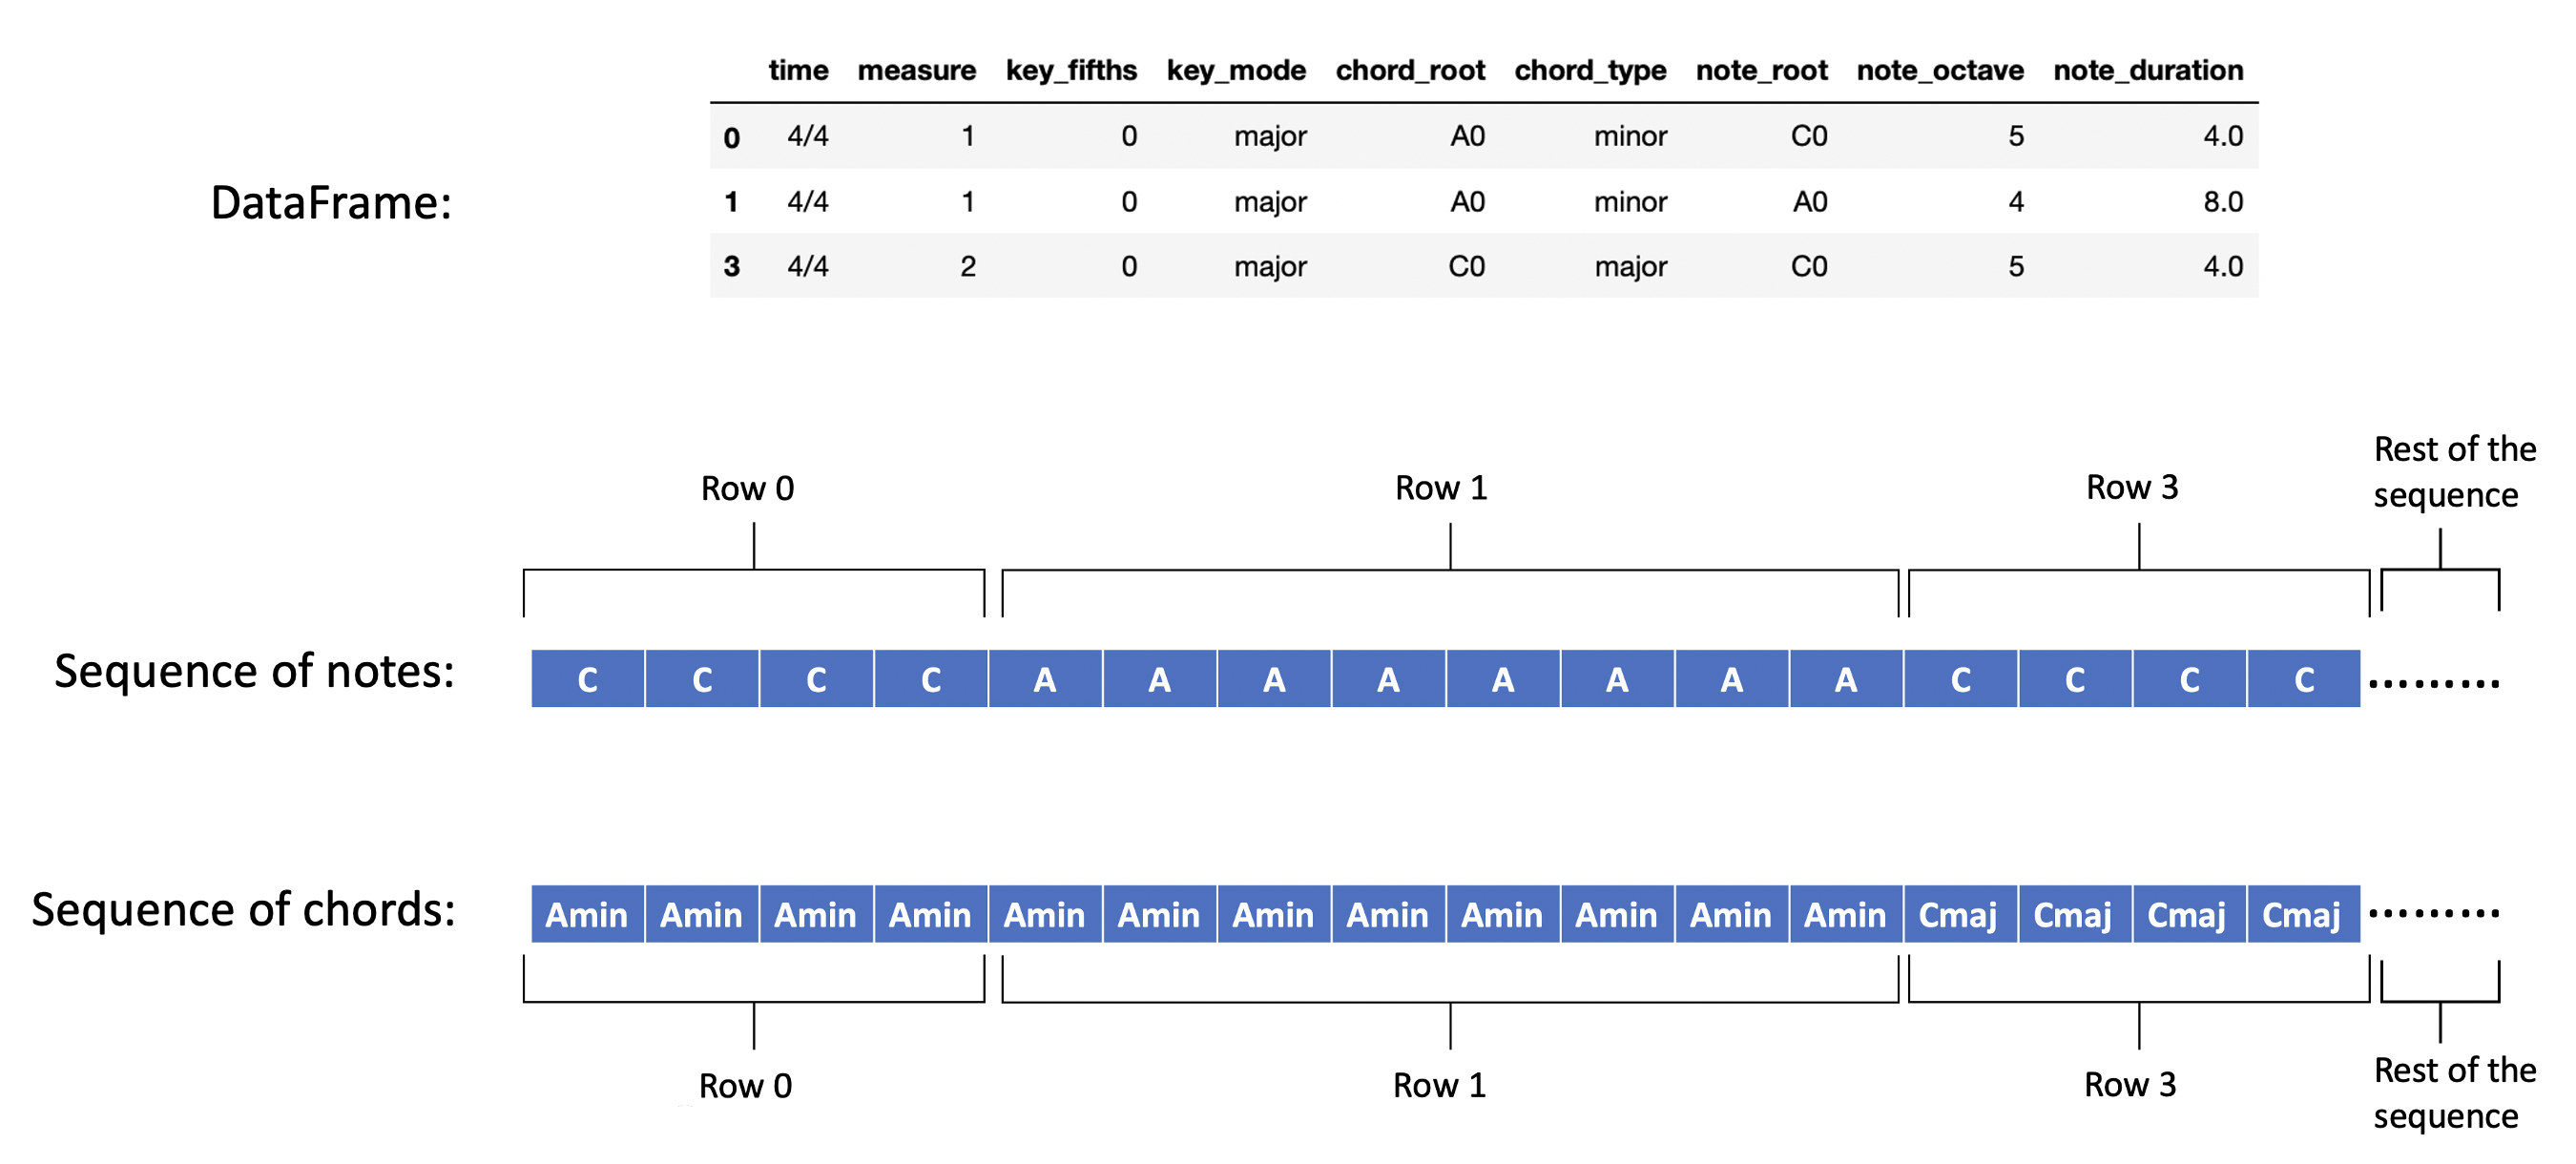
\includegraphics[scale=0.3]{Figures/TransformerData}
    \decoRule
    \caption{Converting DataFrame to Transformer data input format.}
    \label{fig:Transformer training}
    \end{figure}

\begin{figure}
    \centering
    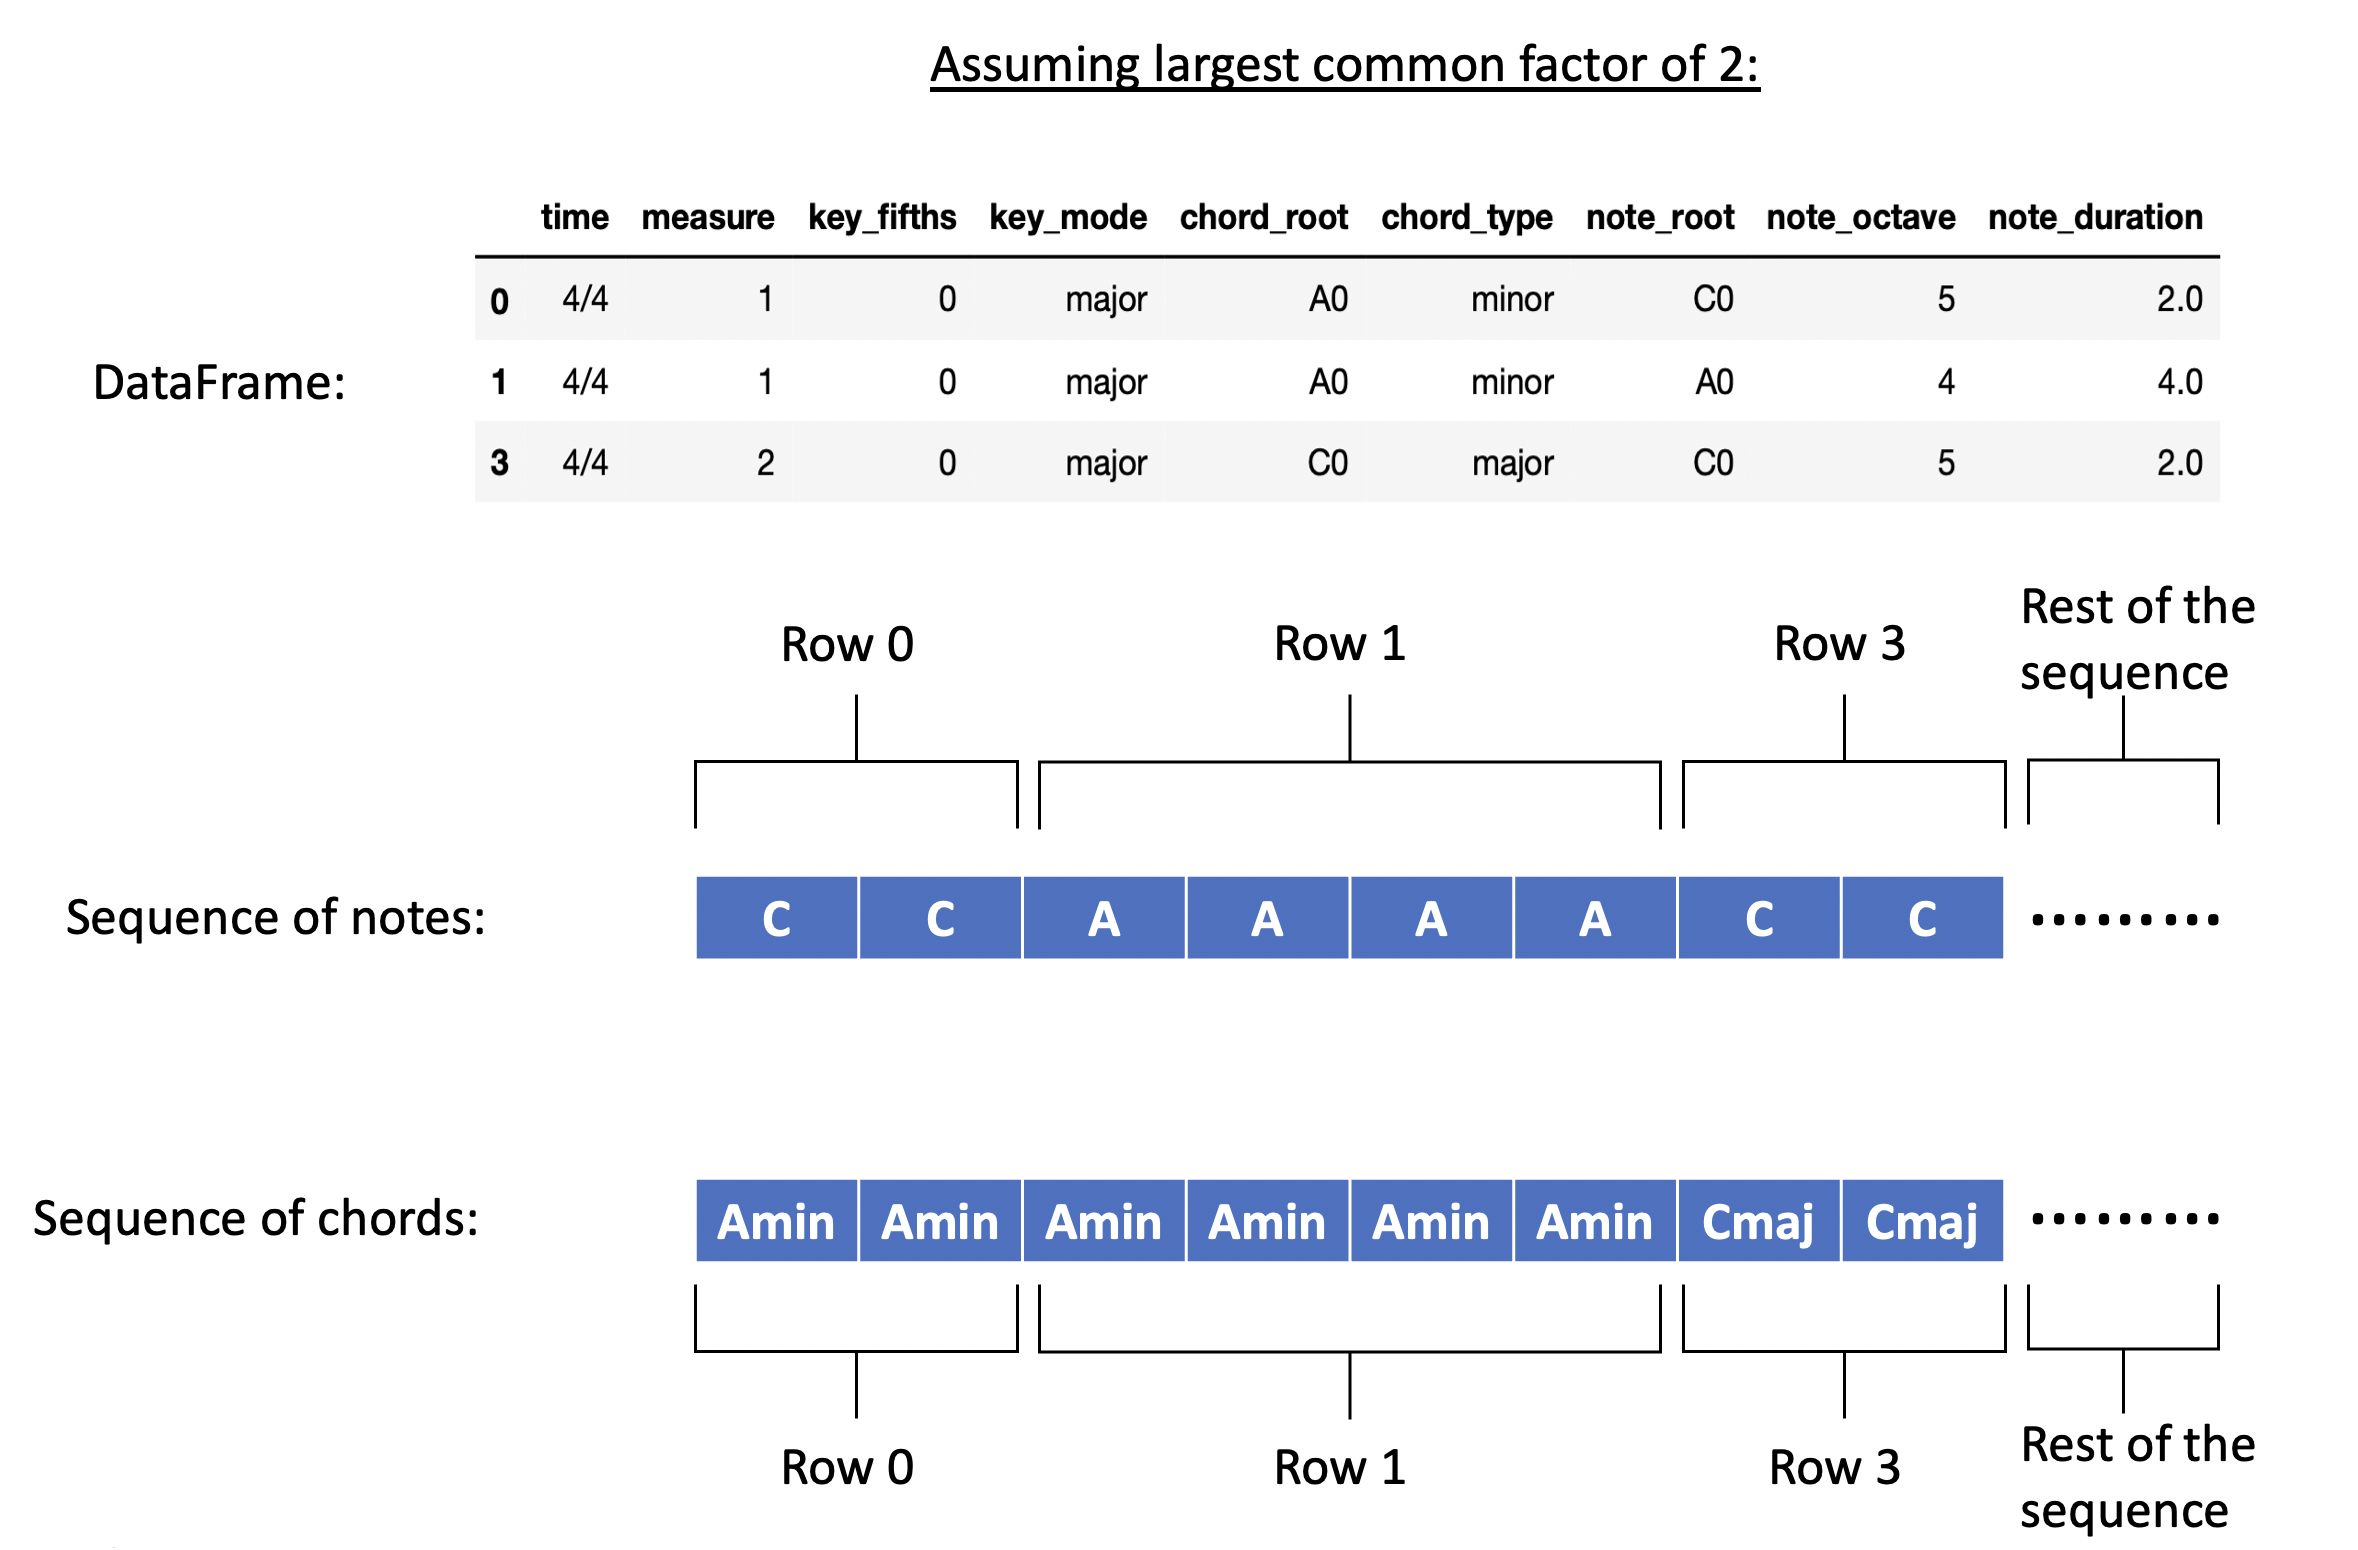
\includegraphics[scale=0.3]{Figures/Transformer LCF}
    \decoRule
    \caption{Converting DataFrame (normalised by the largest common factor) to Transformer data input format.}
    \label{fig:Transformer LCF}
    \end{figure}

\subsubsection{Code}
The same nested loop as before is used again for this. Four empty lists \emph{note\_duration\_li}, \emph{note\_li}, \emph{chord\_li}, \emph{chordtype\_li} are initialised. As we loop through the DataFrame rows of a single song, we append the information from each row to the respective lists. At the end of this inner loop, the largest common factor of \emph{note\_duration\_li} can be found using the \emph{math.gcd} function:

\begin{lstlisting}[language=Python]
    lcf = note_duration_li[0]   #Initialise lcf
    n = len(note_duration_li)   #Number of elements in list
    
    for j in range(1,n):
        lcf = math.gcd(lcf,note_duration_li[j])
\end{lstlisting}


Since \emph{math.gcd} only accepts two arguments, we initialise \emph{lcf} as the index 0 element of \emph{note\_duration\_li}, and loop from the index 1 element to the last element of \emph{note\_duration\_li}. Within this loop, \emph{math.gcd} takes in \emph{lcf} and \emph{note\_duration\_li}[\emph{j}] as its two arguments, where \emph{j} is the correct loop index. In essence, we are just finding the largest common factor of the first two elements of \emph{note\_duration\_li}, and finding the largest common factor of the previous largest common factor and the third element, and so on. This will give us the largest common factor of all the values stored in \emph{note\_duration\_li}, which are all then divided by this largest common factor to give \emph{normalised\_note\_duration}.

We can now start to construct the sequences of notes and chords. Two empty arrays \emph{row\_note} and \emph{row\_chord} are initialised, and we loop through \emph{normalised\_note\_duration} with loop index \emph{k}. For the \emph{k}\textsuperscript{th} element of \emph{normalised\_note\_duration}, a 1 by \emph{normalised\_note\_duration}[\emph{k}] array filled with '1's is initialised and multiplied by \emph{note\_li}[\emph{k}]. The result is concatenated with \emph{row\_note} along the column axis. For the chord sequence, a 1 by \emph{normalised\_note\_duration}[\emph{k}] array filled with '1's is also initialised. This array is multiplied by \emph{chord\_li}[\emph{k}] if chordtype\_li[\emph{k}] is 'major', by $(\emph{chord\_li}[\emph{k}] + 12)$ if it is 'minor', and zero if there are no chords. The resulting array is then concatenated with \emph{row\_chord} along the column axis.

After looping through all the DataFrame rows of a song, \emph{row\_note} and \emph{row\_chord} are the now complete sequences of notes and chords respectively for that song. These will be the input to the Transformer model.

\subsubsection{Sanity Check of code}
We expect the number of elements in each of the note/chord sequence to be less than or equal to the sum of all \emph{note\_duration} for a single song. It will be 'less than' if all the \emph{note\_duration}s have a largest common factor greater than 1.0. Indeed, we see that this is the case for all 4504 note/chord sequences (twice the number of songs in the dataset since we are splitting each song into a separate note and chord sequence) in Figure \ref{fig:Transformer check}.

Again, we manually check a random selection of sequences like we did in the sanity check for the LSTM in Chapter \ref{lstm check}.

\begin{figure}
    \centering
    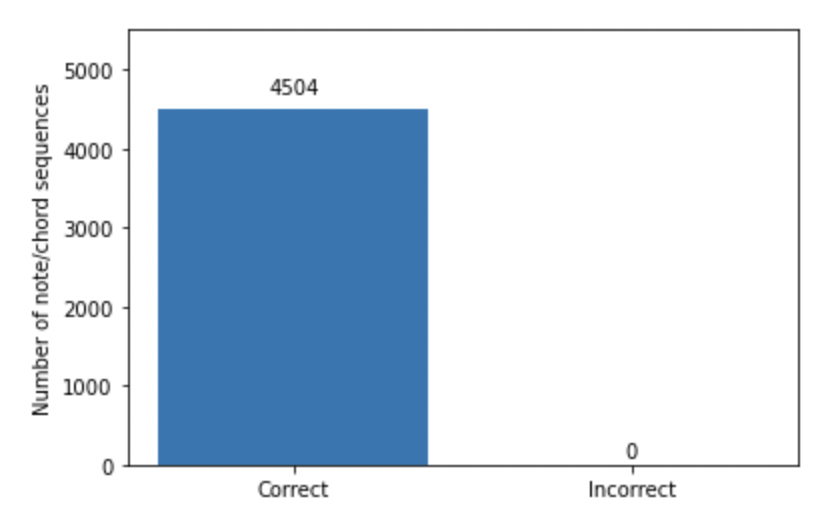
\includegraphics{Figures/Transformer check}
    \decoRule
    \caption{Number of note/chord sequences with 'correct' and 'incorrect' number of columns.}
    \label{fig:Transformer check}
    \end{figure}


\section{Data processor}
\label{data processor}
As can be seen in the last block of \autoref{flowchart}, the data processor receives three pieces of information from the voice processor: note, note duration, and music key. Hence, the preprocessing needed is similar to the one in Section \ref{preprocessing} but simplified:

\begin{enumerate}
    \item Convert the notes to their numerical representations using Table \ref{tab:note_map} to obtain $n_r$.
    \item Since we have the music key information, we can find Pitch 1 of that key using Table \ref{tab:bigtable} to obtain $p_1$.
    \item We now have $n_r$ and $p_1$ and can use Equation \ref{shift note 2} to transpose the notes to C major key.
    %\item Normalise the time signatures by multiplying each note duration with the reciprocal of the time signature to give a normalised note duration.
    \item The preprocessed information is then converted into the LSTM or Transformer format. Note that we needed to provide the chord information to the model when training it, but once trained, the model is meant to output the chords themselves in actual operation. Hence, the data format for the data processor will differ from the data format for the training phase in that the former will only include note information and not chord information.
    \item The fully processed input data is passed to the machine learning model.
  \end{enumerate}

  \subsection{LSTM format}
Since the chord information is no longer needed, the last 25 columns are now irrelevant. Hence, the input data is just a matrix with 12 columns as shown in Figure \ref{fig:LSTM data processor}. Notice the difference between Figure \ref{fig:LSTM data processor} and Figure \ref{fig:LSTM training}.

\begin{figure}
    \centering
    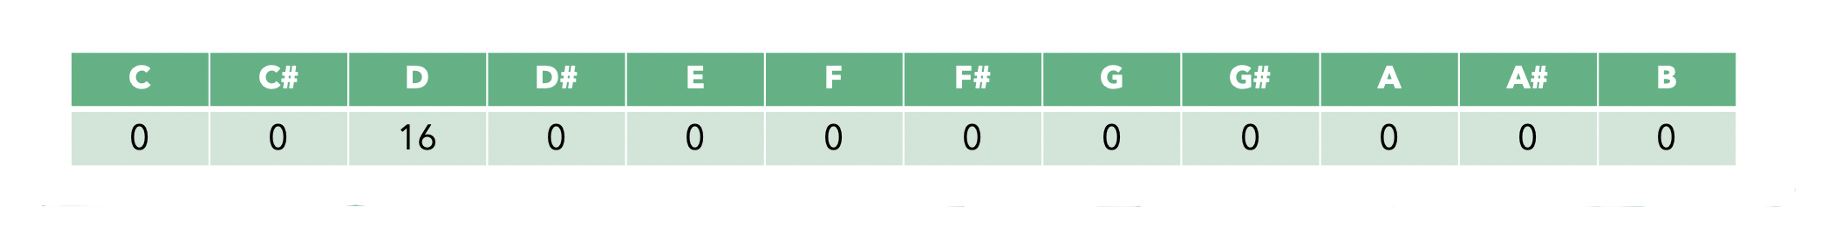
\includegraphics[scale=0.3]{Figures/LSTM data processor}
    \decoRule
    \caption{LSTM data input format (for a single measure) for data processor}
    \label{fig:LSTM data processor}
    \end{figure}

\subsection{Transformer format}
Similarly, we no longer have a sequence of chords since the chord information is presumably not known. This just leaves the sequence of notes, as shown in Figure \ref{fig:Transformer data processor}. Note the difference between Figure \ref{fig:Transformer data processor} and Figure \ref{fig:Transformer LCF}.

\begin{figure}
    \centering
    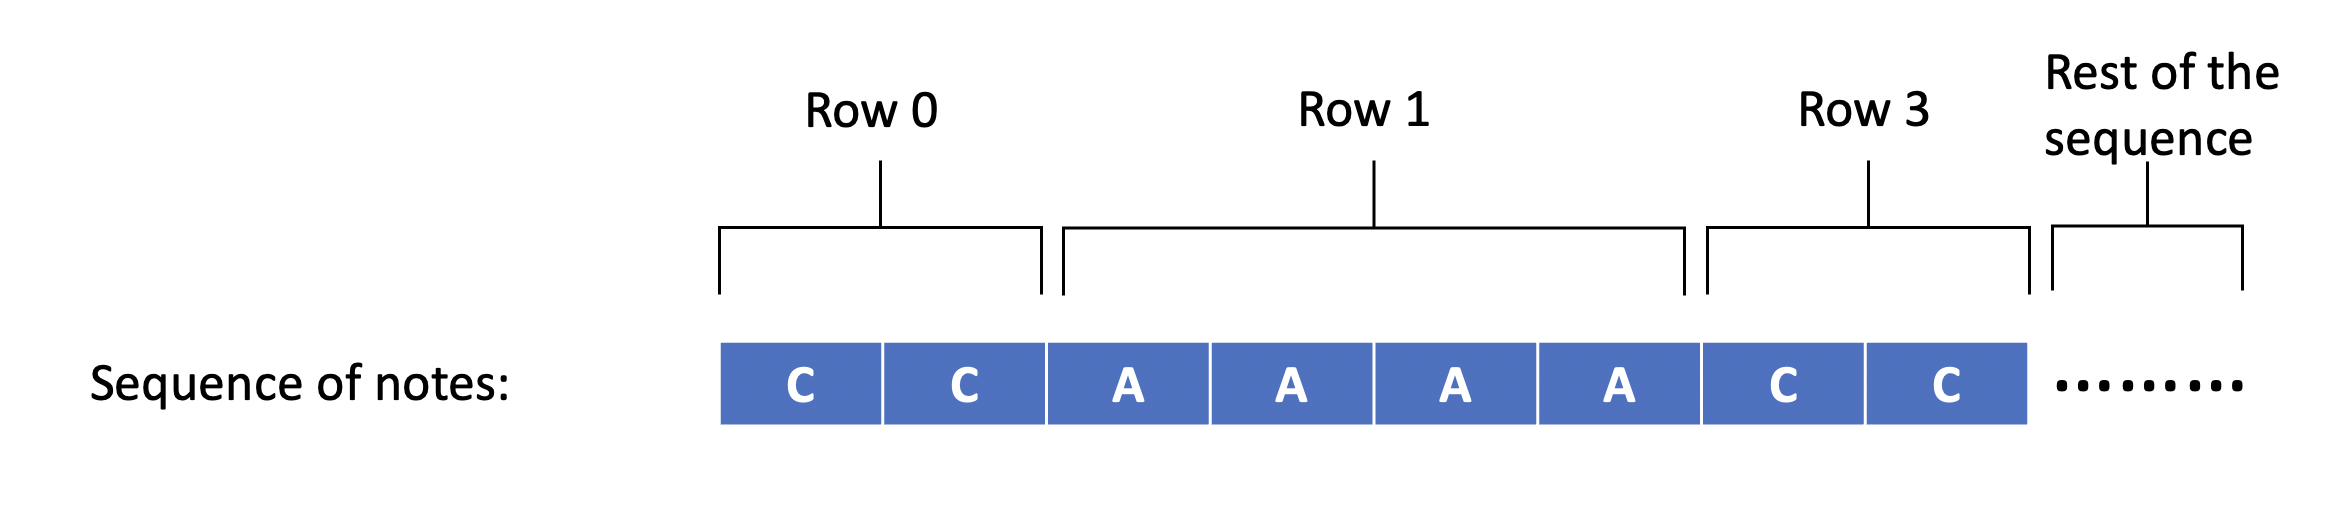
\includegraphics[scale=0.3]{Figures/Transformer data processor}
    \decoRule
    \caption{Transformer data input format for data processor}
    \label{fig:Transformer data processor}
    \end{figure}

\section{Music Mood Classification}
\label{Music Mood Classification}
Everything discussed above in this chapter is crucial to the creation of our Minimum Viable Product. However, there are additional features that we could add to our product if it proves to be successful. As mentioned in \textbf{REFERENCE MOSCOW?} and under the Technological heading in \autoref{STEEP Drivers}, one possible additional functionality would be allowing users to select the music mood of the generated chords, or perhaps even have our machine learning model be able to identify the mood of their singing. This means that our model would need to be trained to identify music moods, which would require mood information in the training dataset. While datasets with expert annotations of music moods exist \cite{allmusic}, it would be useful to be able to assign a music mood to a song ourselves using some sort of algorithm or model.

%\subsection{Human annotations}

%\subsection{Machine learning model annotations}

Classifying the music mood of songs using machine learning models has been a prominent problem in the Music Informatics Research (MIR) community for years \cite{MIRMood}. There are generally two approaches to this problem: regressing a continuous mood space, or treating it as a multi-label classification problem. The latter seems to perform better when working with listener data rather than just the audio content \cite{ListeningData}. Unfortunately, listener data would be difficult to obtain as it is valuable information that corporations would be unlikely to divulge. Additionally, our model will mainly be dealing with newly created song for which listener data will not be available. Hence, an audio-based approach will be our only option if we are to use a machine learning model for mood classification. This leaves us with the continuous mood space.

%\subsubsection{Continuous mood space}

The continuous mood space can be regressed and then clustered to obtain specific moods. This would require an appropriate continuous mood space model.

First, we have the Arousal-Valence model \cite{circumplex}, which is a well-known model in the field of psychology and cognitive science \cite{circumplexbook} \cite{circumplex3}. This model displays emotions on a two-dimensional plane with valence (positive and negative degree of emotion) and arousal (intensity of emotion) as its two axes. Emotions are placed on the two-dimensional model based on their valence and arousal. This model is shown in Figure \ref{fig:circumplex}.

Next, we have Thayer's model, which applies the Arousal-Valence model to music. The main difference is the two axes, with Energy (the volume of the music) and Stress (tonality and tempo of the music) now corresponding to Arousal and Valence. Depending on the level of Energy and Stress, music can be classified into four clusters: Exuberance, Anxious, Contentment, and Depression. This model can be seen in Figure \ref{fig:Thayers}.

Lastly, we have the Tellegen-Watson-Clark model \cite{Watson1985} \cite{Tellegen1999}, which uses positive/negative affect, engagement/disengagement, and pleasantness/unpleasantness to classify music moods. This allows the model to classify a greater variety of music moods than the Arousal-Valence model and the Thayer's model. The Tellegen-Watson-Clark model is shown in Figure \ref{fig:TWC}.

Given that it can classify the greatest variety of music moods, the Tellegen-Watson-Clark model would be the desired model should we decide to tackle the music mood classification problem with a continuous mood space approach. 

\begin{figure}
    \centering
    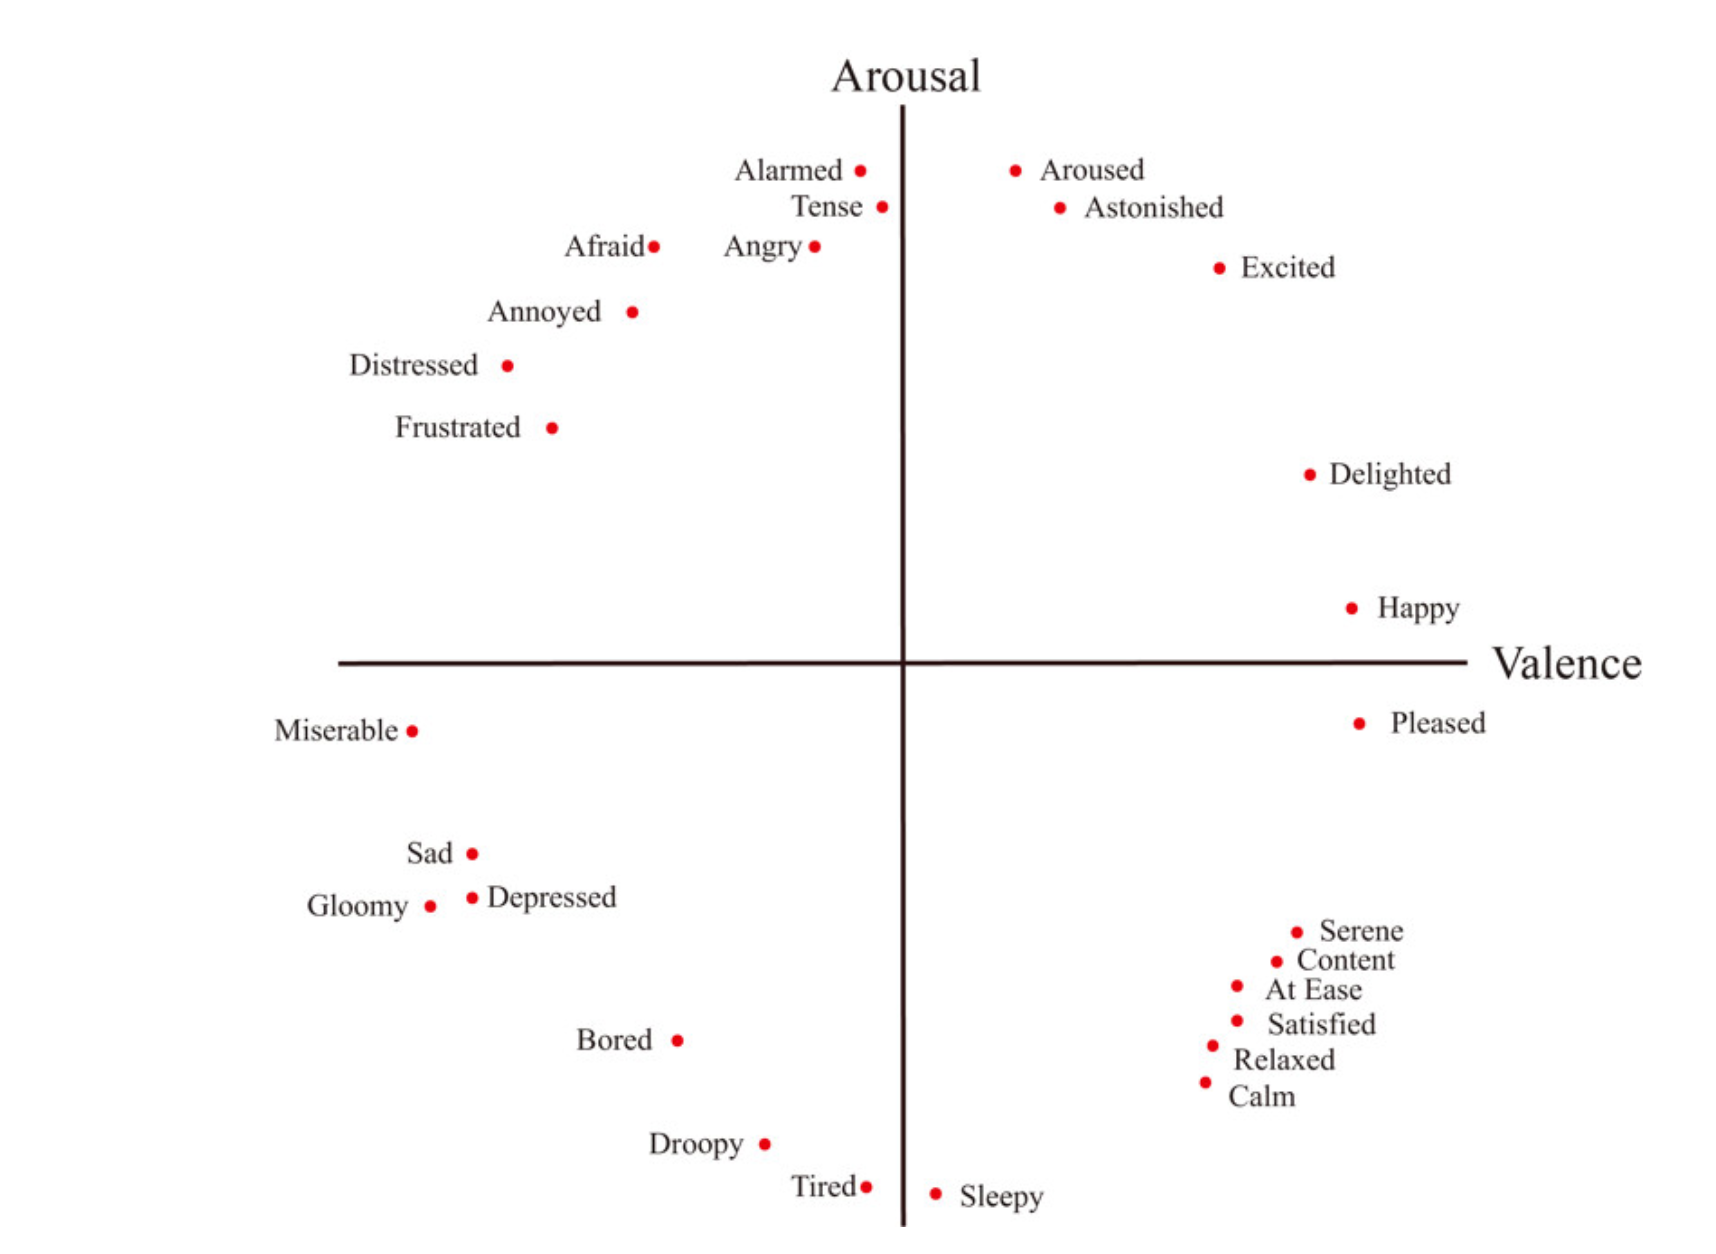
\includegraphics[scale=0.4]{Figures/Arousal-Valence model}
    \decoRule
    \caption{Arousal-Valence model from \cite{MoodIoT}}
    \label{fig:circumplex}
    \end{figure}


\begin{figure}
    \centering
    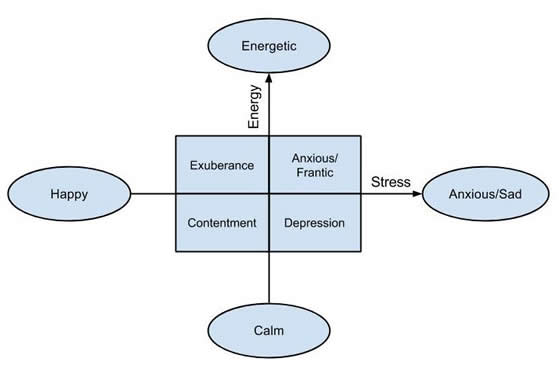
\includegraphics[scale=0.4]{Figures/Thayers model}
    \decoRule
    \caption{Thayer's model from \cite{circumplexbook}}
    \label{fig:Thayers}
    \end{figure}

\begin{figure}
    \centering
    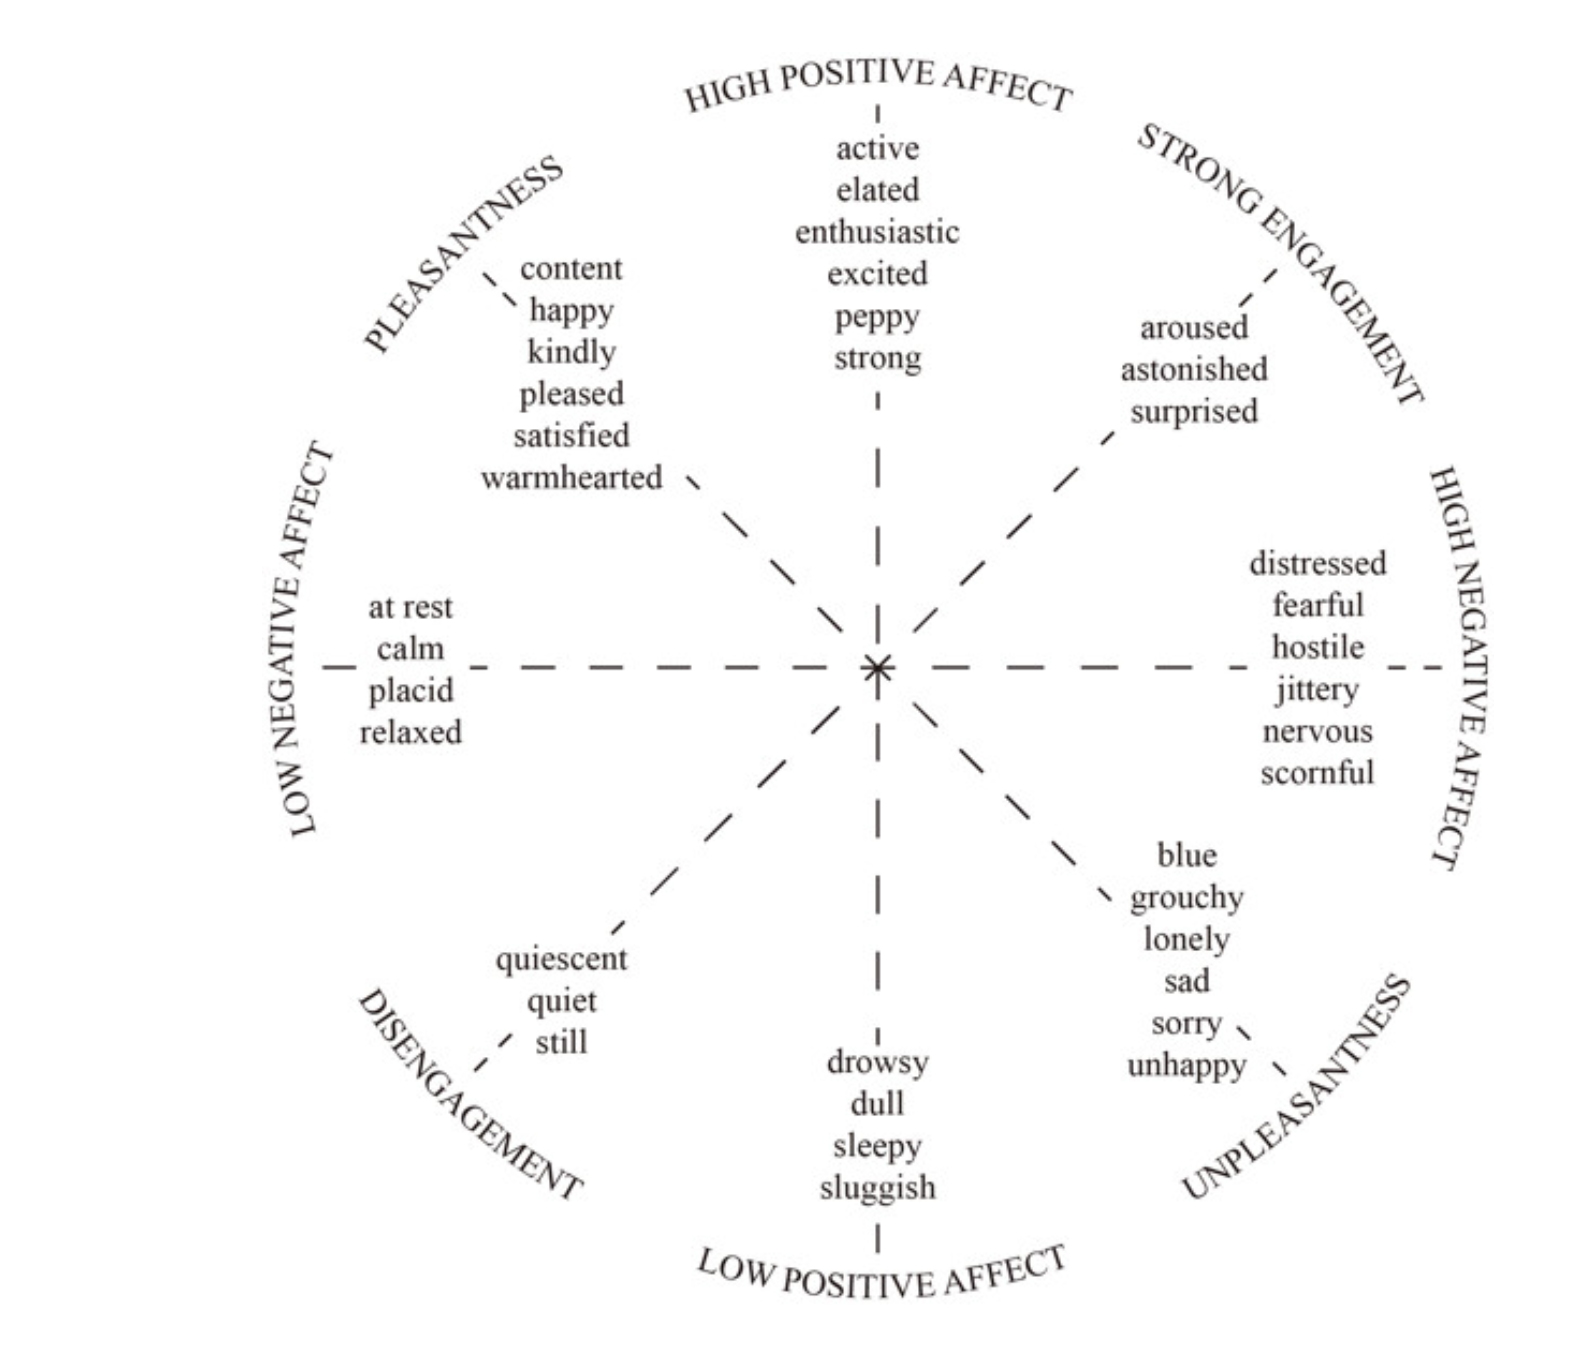
\includegraphics[scale=0.4]{Figures/TWC model}
    \decoRule
    \caption{Tellegen-Watson-Clark model from \cite{MoodIoT}}
    \label{fig:TWC}
    \end{figure}

As for the machine learning model, we would use a Support Vector Machine, which is a classification algorithm. When tested against other popular classification algorithms such as deep neural network \cite{MoodDeepNeuralNetwork}, random forest \cite{Moodrandomforest}, and K-nearest neighbour \cite{MoodKNeighbour} \cite{MoodDeepNeuralNetwork}, the Support Vector Machine was found to be the most accurate at classifying music moods \cite{MoodIoT}.

\section{Summary}

In this chapter, we started by looking at the dataset used to train and test the machine learning model in \autoref{Intro to Dataset} . We then went through the preprocessing steps for the dataset in \autoref{preprocessing}, as well as the conversion into formats that can be fed into a LSTM and a Transformer in \autoref{Model input format}; these are the only sections in this chapter that have actually been implemented. 

In \autoref{data processor}, we looked at the data processor which takes in data from the voice processor and produces input data that is then fed into the machine learning model, as illustrated in \autoref{fig:MVPOverview}. Lastly, we explored the possibility of adding a music mood selection feature in our product, which would require our training/testing dataset to include music mood information. While we could datasets with human annotations of music mood, we explored the possibility of using an algorithm to classify music moods based on audio features. We concluded that using a Support Vector Machine in conjunction with the Tellegen-Watson-Clark model would probably produce the best results.

In the next chapter, we shall look at the actual machine learning models which, as mentioned earlier, receives the output from the data processor.